% Created 2024-05-13 Mon 14:24
% Intended LaTeX compiler: pdflatex
\documentclass[11pt]{article}
\usepackage[utf8]{inputenc}
\usepackage[T1]{fontenc}
\usepackage{graphicx}
\usepackage{longtable}
\usepackage{wrapfig}
\usepackage{rotating}
\usepackage[normalem]{ulem}
\usepackage{amsmath}
\usepackage{amssymb}
\usepackage{capt-of}
\usepackage{hyperref}
\usepackage{minted}
\usepackage[russian]{babel}
\author{cofeek-codes}
\date{13.05.24}
\title{Api в Laravel}
\hypersetup{
 pdfauthor={cofeek-codes},
 pdftitle={Api в Laravel},
 pdfkeywords={},
 pdfsubject={},
 pdfcreator={Emacs 28.2 (Org mode 9.5.5)}, 
 pdflang={Russian}}
\begin{document}

\maketitle
\tableofcontents

\begin{center}
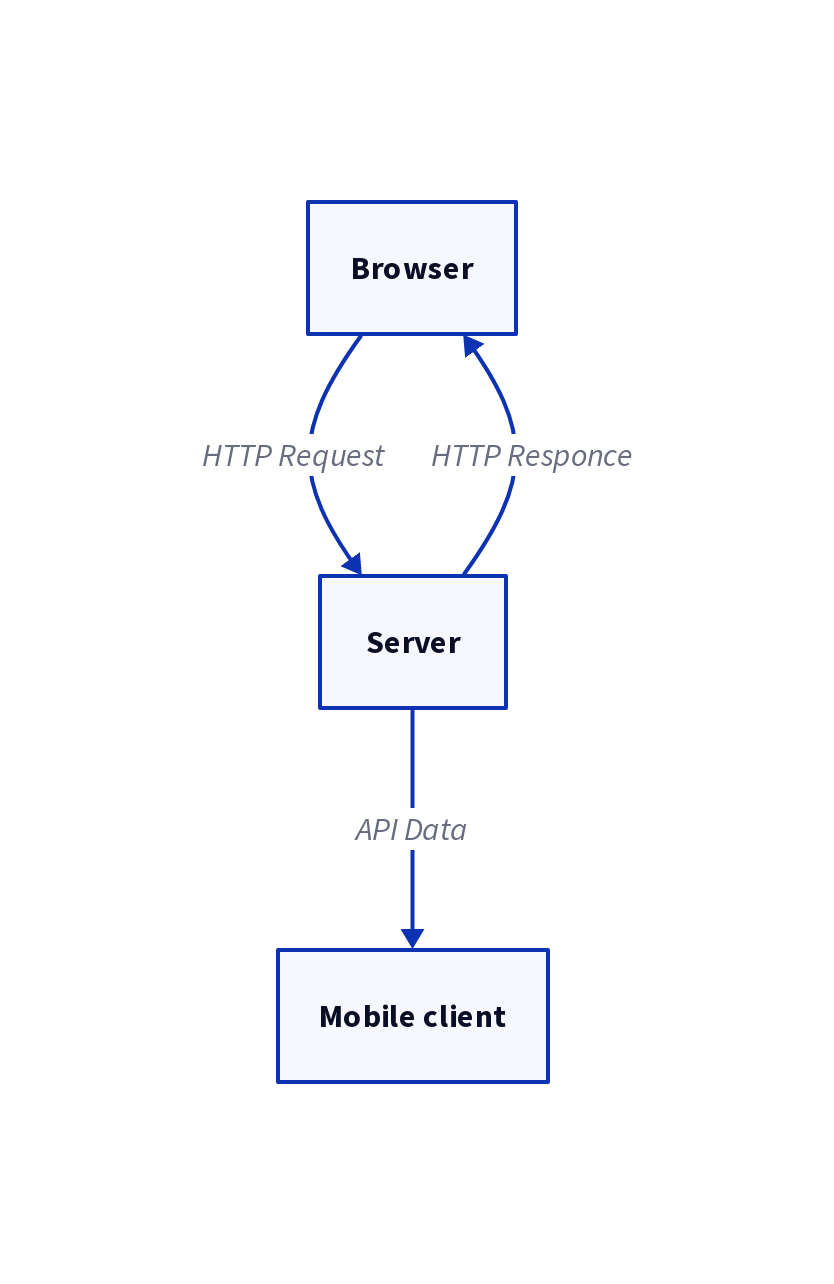
\includegraphics[width=.9\linewidth]{./api.png}
\end{center}


\textbf{Api} - прикладной программный интерфейс, позволяет передавать только данные в форматах \texttt{json/xml/text} между различными компонентами системы
\end{document}